%---------------------------------------------------------------------

                     \begin{frame}
     \frametitle{How to Establish Unsatisfiability?}

Completess is formulated in terms of \alert{derivability} of the empty
clause $\emptyclause$ from a set $S_0$ of clauses in an inference system
$\isI$. However, this
formulations gives \Blue{no hint on \alert{how} to search} for such a
derivation.

\medskip

\visible<2->{
  Idea:

  \begin{itemize}
  \item Take a set of clauses $S$ (the \OliveGreen{search space}),
    initially $S = S_0$.
    \Blue{Repeatedly apply inferences} in $\isI$ to clauses in $S$ and add their
    conclusions to $S$, unless these conclusions are already in $S$.
  \item If, at any stage, we obtain $\emptyclause$, we terminate and
    \Blue{report unsatisfiability} of $S_0$. 
  \end{itemize}
}

                               \end{frame}


%---------------------------------------------------------------------

                     \begin{frame}
     \frametitle{How to Establish Satisfiability?}

When can we report \alert{satisfiability}?

\medskip

\vs<2->{
  When we build a set $S$ such that any inference applied to clauses
  in $S$ is already a member of $S$. Any such set of clauses is called
  \alert{saturated} (with respect to $\isI$).
}

\medskip

\vs<3->{
  In first-order logic it is often the case that all saturated sets
  are infinite (due to undecidability), so in practice we can never
  build a saturated set.

\medskip

  The process of trying to build one is referred to as
  \alert{saturation}.
}

                                \end{frame}


%---------------------------------------------------------------------

	   \begin{frame}\frametitle{Saturated Set of Clauses}

  Let $\M{\isI}$ be an inference system on formulas and $\M{S}$ be a set of 
  formulas. 

\begin{itemize}
\item
$\M{S}$ is called \DI{saturated with respect to $\M{\isI}$}{saturated},
  or simply \alert{$\M{\isI}$-saturated},
  if for every inference of $\M{\isI}$ with premises in $\M{S}$, the conclusion
  of this inference also belongs to $\M{S}$.

\item 
The \DI{closure of $\M{S}$ with
  respect to $\M{\isI}$}{closure!with respect to inference inference system},
  or simply \DI{$\M{\isI}$-closure}{closure!$\M{\protect\isI}$-},
  is the smallest set $\M{S'}$ containing $\M{S}$ and saturated with respect to
  $\M{\isI}$.
\end{itemize}

                           \end{frame}

%---------------------------------------------------------------------

	   \begin{frame}\frametitle{Inference Process}

  \alert{Inference process:} sequence
  of sets of formulas $\M{S_0,S_1,\ldots}$, denoted by 

    \[
      \M{S_0 \RR S_1 \RR S_2 \RR \ldots}
    \]
  $\M{(S_i \RR S_{i+1})}$ is a \DI{step}{step!of inference process} of this 
  process. 

\medskip

\vs<2->{
   We say that this
  step is an \DII{$\M{\isI}$-step}{$\M{\protect\isI}$-step}{step!$\M{\protect\isI}$-} if

  \begin{enumerate}
  \item there exists an inference

    \[\M{
      \infer{F}{F_1 & \ldots & F_n}
    }\]
    in $\M{\isI}$ such that $\M{\setof{\xone{F}{n}} \subseteq S_i}$;

  \item $\M{S_{i+1} = S_i \cup \setof{F}}$.
  \end{enumerate}
}

\medskip

\vs<3->{
  An \DI{$\M{\isI}$-inference process}{inference process!$\M{\protect\isI}$-}
  is an inference process whose every step is an $\M{\isI}$-step.
}

                           \end{frame}

%---------------------------------------------------------------------

	   \begin{frame}\frametitle{Property}

  Let $\M{S_0 \RR S_1 \RR S_2 \RR \ldots}$ be an $\M{\isI}$-inference process
  and a formula $\M{F}$ belongs to some $\M{S_i}$. Then $\M{F}$ is derivable in
  $\M{\isI}$ from $\M{S_0}$. In particular, every $\M{S_i}$ is a subset of the
  $\M{\isI}$-closure of $\M{S_0}$.


                           \end{frame}
\end{document}
%---------------------------------------------------------------------

	   \begin{frame}\frametitle{Limit of a Process}

The \DI{limit}{limit of inference process} of an inference process
$\M{S_0 \RR S_1 \RR S_2 \RR \ldots}$
is the set of formulas $\M{\bigcup_i S_i}$.

\medskip

\vs<2->{
  In other words, the limit is \alert<2>{the set of all derived formulas}.
}

\medskip

\vs<3->{
  Suppose that we have an infinite inference process such that $S_0$
  is \Blue{unsatisfiable} and we use the \Blue{binary resolution
    inference system}. 
}

\bigskip

\vs<4->{
  \alert{Question}: does completeness imply that the limit of the process
  contains the empty clause?  
}

                           \end{frame}

%---------------------------------------------------------------------

	   \begin{frame}\frametitle{Fairness}

  Let $\M{S_0 \RR S_1 \RR S_2 \RR \ldots}$ be an inference process with
  the limit $\M{S_\omega}$. The process 
  is called \DI{fair}{fair!inference process} if for every 
  $\M{\isI}$-inference

    \[\M{
      \infer[,]{F}{F_1 & \ldots & F_n}
    }\]
  if $\M{\setof{\xone{F}{n}} \subseteq S_\omega}$, then
  there exists $\M{i}$ such that $\M{F \in S_i}$.


                           \end{frame}

%---------------------------------------------------------------------

        	   \begin{frame}\frametitle{Completeness, reformulated}

\textbf{\OliveGreen{Theorem}}
Let $\M{\isI}$ be an inference system.
The following conditions are equivalent.

\begin{enumerate}
\item $\M{\isI}$ is complete.
\item For every unsatisfiable set of formulas $\M{S_0}$ and any
  fair $\M{\isI}$-inference process with the initial set $\M{S_0}$, 
  the limit of this inference process contains $\M{\emptyclause}$.
\end{enumerate}

                           \end{frame}

%---------------------------------------------------------------------

	    \begin{frame}\frametitle{Fair Saturation Algorithms:
                Inference Selection by Clause Selection}


\begin{center}
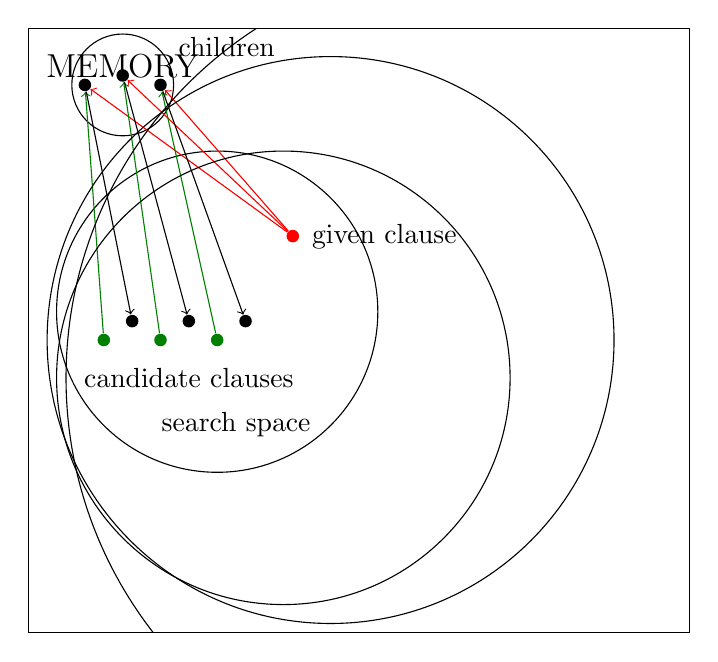
\begin{tikzpicture}[scale=0.12]
\clip[draw] (-20,-34) rectangle (50,30);
\vs<1-6>{\draw (0,0) circle(17);}
\node at (2,-12) {\Blue{search space}};
\vs<2-4,8-10>{\node[fill=red,circle,inner sep=1.6] (g) at (8,8) {};}
\vs<2-4,8-10>{\node[right] at (9,8) {\alert{given clause}};}
\vs<3-4,9-10>{\node at (-3,-7) {\Green{candidate clauses}};}
\vs<3-4,9-10>{\node[fill=Green,circle,inner sep=1.6] (cc1) at (-12,-3) {};}
\vs<3-4,9-10>{\node[fill=Green,circle,inner sep=1.6] (cc2) at (-6,-3) {};}
\vs<3-4,9-10>{\node[fill=Green,circle,inner sep=1.6] (cc3) at (0,-3) {};}
\vs<4-6,10-12>{\node at (1,28) {children};}
\vs<4-6,10-12>{\node[fill=black,circle,inner sep=1.6] (c3) at (-6,24) {};}
\vs<4-6,10-12>{\node[fill=black,circle,inner sep=1.6] (c2) at (-10,25) {};}
\vs<4-6,10-12>{\node[fill=black,circle,inner sep=1.6] (c1) at (-14,24) {};}
\vs<4-6,10-12>{\node[draw,circle,inner sep=13] at (-10,24) {};}
\vs<4,10>{\draw[->,red] (g)--(c1);}
\vs<4,10>{\draw[->,red] (g)--(c2);}
\vs<4,10>{\draw[->,red] (g)--(c3);}
\vs<4,10>{\draw[->,Green] (cc1)--(c1);}
\vs<4,10>{\draw[->,Green] (cc2)--(c2);}
\vs<4,10>{\draw[->,Green] (cc3)--(c3);}
\vs<6,12>{\node[fill=black,circle,inner sep=1.6] (ca1) at (-9,-1) {};}
\vs<6,12>{\node[fill=black,circle,inner sep=1.6] (ca2) at (-3,-1) {};}
\vs<6,12>{\node[fill=black,circle,inner sep=1.6] (ca3) at (3,-1) {};}
\vs<6,12>{\draw[->] (c1)--(ca1);}
\vs<6,12>{\draw[->] (c2)--(ca2);}
\vs<6,12>{\draw[->] (c3)--(ca3);}
\vs<7-12>{\draw (7,-7) circle(24);}
\vs<13>{\draw (12,-3) circle(30);}
\vs<14->{\draw (28,-7) circle(44);}
\vs<15->{\node at (-10,26) {\alert{\large{MEMORY}}};}
\end{tikzpicture}
\end{center}



                              \end{frame}



%---------------------------------------------------------------------

                       \begin{frame}\frametitle{Saturation Algorithm}

A \alert{saturation algorithm} tries to \Fuchsia{saturate} 
a set of clauses with  respect to a given inference system.

\Blue{In theory} there are three possible scenarios:

\begin{enumerate}
  \item At some moment the empty clause $\M{\emptyclause}$ is generated,
  in this case the input set of clauses is unsatisfiable.

  \item Saturation will terminate without ever 
  generating $\M{\emptyclause}$, in this
  case the input set of clauses in satisfiable.

  \item Saturation will run \alert{\underline{forever}}, but without generating $\M{\emptyclause}$. In
  this case the input set of clauses is \Blue{\underline{satisfiable}}.
\end{enumerate}

                               \end{frame}


%---------------------------------------------------------------------

                \begin{frame}\frametitle{Saturation Algorithm in Practice}

\Blue{In practice} there are three possible scenarios:

\begin{enumerate}
  \item At some moment the empty clause $\M{\emptyclause}$ is generated,
  in this case the input set of clauses is unsatisfiable.

  \item Saturation will terminate without ever 
  generating $\M{\emptyclause}$, in this
  case the input set of clauses in satisfiable.

  \item Saturation will run \alert{\underline{until we run out of resources}}, 
  but without generating $\M{\emptyclause}$. In
  this case it is 
 \Blue{\underline{unknown}} whether the input set is unsatisfiable.
\end{enumerate}

                               \end{frame}
